
\chapter{Implementation}

In section \ref{sec:challenges} we presented the three main challenges of this research paper: portability, security and speed. To accurately assess whether the design presented in chapter \ref{chap:solution} meets these challenges, an example system was implemented by the researchers of this paper. This chapter is devoted to illustrating the various aspects of this implementation, serving as a platform that is subject to evaluation in the next chapter. First, the individual pieces of hardware that were used in the implementation are discussed. Second, set-up of the demo in general is explained. In the last section of this chapter, the implementations of the three key aspects of section \ref{sec:obd2_access_control} are illustrated.

\section{Hardware}
\label{sec:hardware}
It is clear that the design presented in chapter \ref{chap:solution}, as well as the OBD-II system is general, is of an embedded nature. The gateway ECU is embedded by default, since it is implemented by a microcontroller in all extant intra vehicle networks. The tester device however, introduced by the researchers of this paper, could be either implemented by an embedded device (e.g. tester) or a software application running on a standard PC (e.g. a laptop owned by the repair shop) that is connected to the OBD-II port via some adapter. The decision was made to implement the former (i.e. the tester is also embedded). Because of this decision, the tester and gateway can be implemented on the same microcontroller architecture. This means that the same CAN messaging library can be used in both microcontrollers. \\ \\ The microcontroller chosen for our implementation is the Atmel AT90CAN128. It boasts a 128 KB flash memory, 4KB of EEPROM and 4KB SRAM (for more information on these specs see \ref{sec:microcontrollers}). More importantly, it includes a dedicated CAN controller, which allows for easy CAN networking between devices. The DVK90CAN1 is a development kit that includes the AT90CAN128, as well as introducing a series of hardware peripherals like power supply inputs,LEDS, buttons, connectors, transceivers, programming interfaces, debuggers, etc. The ones that were extensively used in our implementation are:
\begin{itemize}
	\item \textbf{Programming/Debugging interface} The DVK90CAN1 includes the option of easily connecting to a standard PC for programming and debugging. This is done by connecting the ATMEL-ICE BASIC programmer to both the DVK90CAN1 board and a PC running Atmel Studio, which is an integrated development platform (IDP) that allows us to run and debug C and assembly code on both microcontrollers.
	
	\item \textbf{CAN Transceiver:} This device functions as a transmitter and receiver by transmitting messages from the CAN controller on to the CAN bus (male DB9), as well as receiving incoming CAN messages and forwarding them to the CAN controller. 
	
	\item \textbf{Male DB9:} This connector belongs to the D-sub series, where the B denotes the shell size and the 9 means there are 9 pins. This connector assumes the CAN bus connections.
	
	\item \textbf{RS-232 driver/receiver:} Recommended standard 232 (RS-232) is a standard for serial transmission of data. The driver/receiver is responsible for transmitting and receiving RS-232 data (female DB-9).
	
	\item \textbf{Female DB9:} This connector assumes the RS-232 connections.
	
	\item \textbf{Compass Card Keyboard} 4 de-centered push-buttons of compass card keyboard are present on the board, allowing for user interactivity.
\end{itemize}
Besides some peripherals offered by the DVK90CAN1 board and the ATMEL-ICE BASIC programmer, two more pieces of hardware were use in our system. First; there's a female-to-female DB9 cable. This is used to connect the CAN interfaces of both boards. Second there's a male-to-male DB9 cable that is connected to a generic RS232 to usb converter. This cable allows both boards to be connected to a PC for serial communications.

\section{Demo Set-Up}
\label{sec:demo_setup}

Figure \ref{fig:demo} shows the set-up of the implementation. One board functions as the tester, which is connected via CAN (using the female-to-female DB9 cable) to the other board, which in turn functions as the gateway. This connection is used to implement the general authentication and message authentication procedures presented in section \ref{subsec:authentication_procedure} and \ref{subsec:message_authentication}. The permission table outlined in section \ref{subsec:sol_permissions_table} is implemented on the gateway. The gateway is also connected to a PC using the RS-232 communications standard to allow for real time feedback (e.g. signalling when a signature verification procedure successfully terminates). The attentive reader might notice two integral components missing from this set-up: the central server that is introduced in section \ref{fig:authentication_procedure}, as well as the intra vehicle network itself. The decision was made to implement these components only logically. This was done for two reasons: first, a realistic implementation of these components would result in the introduction of more hardware, greatly increasing the time and cost required to construct a working demo. Second, since the primary focus of this paper is the RBAC system proposed in chapter \ref{chap:solution}, as well as all the procedures and systems introduced to enforce it (i.e. authentication procedure, message authentication procedure and permissions table), providing a physical central server and intra vehicle network implementation can be considered out of scope. The logical implementation of both these components was done as follows:
\begin{itemize}
	\item \textbf{Central Server:} The software on the tester board implements a dedicated key-API that specifies a series of private key related functions (for signing and calculating the shared secret). As far as the main tester software is concerned, calling these functions could result in a remote server being addressed.
	
	\item \textbf{Intra Vehicle Network:} The RS-232 connection between gateway and PC is used for this purpose. Whenever a message is accepted by the gateway, instead of forwarding the message to another sub-network, a message is transmitted to the PC. This message contains the ID of the accepted message, as well as a line of text signalling that the message was accepted.
\end{itemize}

\begin{figure}[h]
	\label{fig:demo}
	\caption{Hardware set-up that is used to implement the proposed solution.}
\end{figure}

\section{OBD-II Access Control Implementation}
The key aspects aspects of the OBD-II access control system presented in chapter \ref{chap:solution} are the authentication procedure, the message authentication procedure and of course the permissions table. How these were implemented in the set-up presented in section \ref{sec:demo_setup} is discussed next. 

\subsection{Authentication Procedure Implementation}
\label{subsec:authentication_procedure_implementation}

Figure \ref{fig:authentication_procedure_implementation} shows how the authentication procedure was implemented in our demo. Because of our decision to omit the central server and the intra vehicle network, these are naturally not included in the diagram. Because of this, the tester now stores the OBD private key $P_obd$ instead of the central server. In our diagram we have chosen to include the size of this key (in bits)in the superscript: $Pr_{obd}^{256}$. This was repeated for every piece of data in the diagram (e.g. keys and signatures). The corresponding public key is stored on the gateway: $Pb_{obd}^{512}$. The size of these keys was mandated by the decision to guarantee a security level of 128 bits (see \ref{sec:security_level}). As mentioned in section \ref{subsec:ECC}, the decision was made to use elliptic curve asymmetric key pairs. According to \cite{wiki:ECC}, ECC keys have the property that the size of the underlying field (i.e. the size of the key), should be twice the security parameter. The decision was made to work with the secp256r1 curve, which meets our security level guarantee ($\frac{256}{2}=128$) and introduces fixed sizes for our keys (256 bit for the private key and 512 bits for the private key.

\paragraph{The Procedure}

The authentication procedure is initiated by the tester, which transmits an initialisation message to the gateway. This message contains the role that the tester wishes to authenticate as: $Role^8$. Because it is only 8 bits in size, it fits into a single CAN message (remember from section \ref{subsec:can:frames}, figure \ref{fig:CANframe} that a CAN message can hold up to 64 bits of data). The gateway reacts to this message by creating a new ECC keypair: KGen($Pb_g^{512}$,$Pr_g^{256}$. The same curve must be used as the one chosen for the original OBD keys (i.e. secp256r1), otherwise the ECDH secret generation algorithm used later on won't work. As a result of this, both key pairs have the same respective sizes. Next, the newly generated public key $Pb_g^{512}$ is transmitted to the tester. Because of it's size (512 bits), this key won't fit into a single CAN message. This problem is remedied by spreading the key over 8 distinct CAN messages, and sending them to the tester one by one. After the tester receives all 8 messages, and assembles the public key, it will first hash it: SHA512($Pb_g^{512}$), after which the signing function of the key API is called: Sig(SHA512($Pb_g^{512}$),$Pr_{obd}^{256}$). This results in the signature being generated: $S^{512}$. Again the size is mandated by our security level guarantee of 124 bits, since according to \cite{wiki:ECDSA} typical ECDSA signature should be four times the size of the desired security level ($\frac{512}{4}=128$). Once the signature is calculated, it sent to the gateway. Because the signature is the same size as the public key that was sent earlier, it is also spread over 8 different CAN messages. Upon reception, the gateway verifies the validity of the signature by first hashing it with the same hash function used in it's generation (SHA512), before running the ECDSA verification procedure: Ver(SHA512($S^{512}$),$Pb_{obd}^{512}$). If and when the verification is successful, an ACK message is transmitted to the tester. Both tester and gateway can now generate the shared secret: ECDH($Pr_{obd}^{256}$,$Pb_g^{512}$) and ECDH($Pr_g^{256}$,$Pb_{obd}^{512}$), which will be used in the message authentication procedure.

\begin{figure}[h]
	\centering
	\fbox{
		\procedure{OBD-II Authentication Procedure Implementation}{%
			\textbf{Tester}  \<\< \textbf{Gateway} \\
			\text{$Pr_{obd}^{256}$} \<\< \text{$Pb_{obd}^{512}$} \\
			\< \sendmessageright{top=\text{$Role^8$ (1 frame)}} \<\\
			\<\< \text{KGen($Pb_g^{512}$,$Pr_g^{256}$)} \\
			\< \sendmessageleft{top=\text{$Pb_g^{512}$ (8 frames)}} \<\\
			\text{$S^{512}$=Sig(SHA512($Pb_g^{512}$),$Pr_{obd}^{256}$)} \<\<\<\< \\
			\< \sendmessageright{top=\text{$S^{512}$ (8 frames)}} \<\\
			\<\< \text{Ver(SHA512($S^{512}$),$Pb_{obd}^{512}$)} \\
			\< \sendmessageleft{top=\text{$ACK^{8}$ (1 frame)}} \<\\
			\text{$K^{256}$=ECDH($Pr_{obd}^{256}$,$Pb_g^{512}$)} \<\< \text{$K^{256}$=ECDH($Pr_g^{256}$,$Pb_{obd}^{512}$)} \\
		}
	}
	\caption{OBD-II Authentication Procedure Implementation}
	\label{fig:authentication_procedure_implementation}
\end{figure}



\subsection{Message Authentication Procedure Implementation}
\label{subsec:message_authentication_procedure_implementation}

Figure \ref{fig:message_authentication_implementation} shows the implementation of the message authentication procedure. After the procedure from section \ref{subsec:authentication_procedure_implementation} completes, and the shared secret $K$ is established, this procedure is repeated for every OBD-II message sent by the tester. The procedure starts when the tester sends the message $M64$ (again superscript is used to indicate the size). The gateway receives the message and checks the permissions table:  CheckP($M^{64}$(see section \ref{subsec:permissions_table_implementation}), before sending an acknowledgement back to the tester: $ACK^8$. This acknowledgement is positive or negative based on the outcome of the earlier permissions table check. Upon reception of the acknowledgement, the tester calculates the MAC of the message using the shared secret and HMAC\textunderscore SHA256: $Mac^{256}$=Hmac\textunderscore SHA256($M$,$K$)\footnote{To reduce the performance overhead, the MAC can be computed right after sending the original OBD-II message. This would allow the MAC to be ready before the first acknowledgement is received.}. The size of this MAC is again mandated by our security guarantee of 128 bits. This is because the SHA265 cryptographic hash algorithm has a security level of 128 bits against collision attacks. The MAC is then sent to the Gateway, which will in turn verify it using the shared secret: Ver($Mac^{256}$,$K$). If the MAC is valid, the original message $M^{64}$ is forwarded to the intra vehicle network: Forward($M^{64}$), which in our implementation was indicated by sending a RS232 message to a connected PC. The tester is also informed of this by sending another acknowledgement. Upon reception the tester might want to send another message, in which case the entire procedure is repeated. 

\begin{figure}[h]
	\centering
	\fbox{
		\procedure{Message Authentication}{%
			\textbf{Tester}  \<\< \textbf{Gateway} \\
			\text{$K$}  \<\< \text{$K$} \\
			\< \sendmessageright{top=\text{OBD-II message $M^{64}$ (1 frame)}} \<\\
			\<\< \text{CheckP($M^{256}$)} \\
			\< \sendmessageleft{top=\text{$ACK^8$ (1 frame)}} \< \\
			\text{$Mac^{256}$=Hmac\textunderscore SHA256($M$,$K$) } \<\< \\
			\< \sendmessageright{top=\text{$Mac^{256}$} (4 frames)} \<\\
			\<\< \text{Ver($Mac^{256}$,$K$)}  \\
			\<\< \text{Forward($M^{64}$)}  \\
			\< \sendmessageleft{top=\text{$ACK^8$ (1 frame)}} \< \\
		}
	}
	\caption{OBD-II Message Authentication Implementation}
	\label{fig:message_authentication_implementation}
\end{figure}

\subsection{Permissions Table Implementation}
\label{subsec:permissions_table_implementation}

The permissions table is implemented according to the design of section \ref{subsec:permissions_table}. Generally, a permissions table for a RBAC system will use hash functions to map user names to fixed size indices. However, in our case the user names are replaced by CAN message ID's, which already have a fixed size of 11 bits (or 29 if the extended frame format is used), negating the need for any hash functions. Figure \ref{fig:permissions} shows how the permission table was implemented. The upper table lists all the roles currently implemented, as well as their byte representation (This representation is also used in the $Role^{8}$ message of the authentication procedure in section \ref{subsec:authentication_procedure_implementation}). Beneath this, the implementation of the example of table \ref{table:2} is given. Every ID entry points to a data structure consisting of a series of bytes, each one associated with a role. The presence of a certain role in this series of bytes, indicates that this role has the permission to send a message with the aforementioned ID. Permissions are easily granted and revoked (Admin role) by deleting and adding role bytes to the data structure pointed to by the chosen ID. 

\begin{figure}[h]
	\label{fig:permissions}
	\centering
	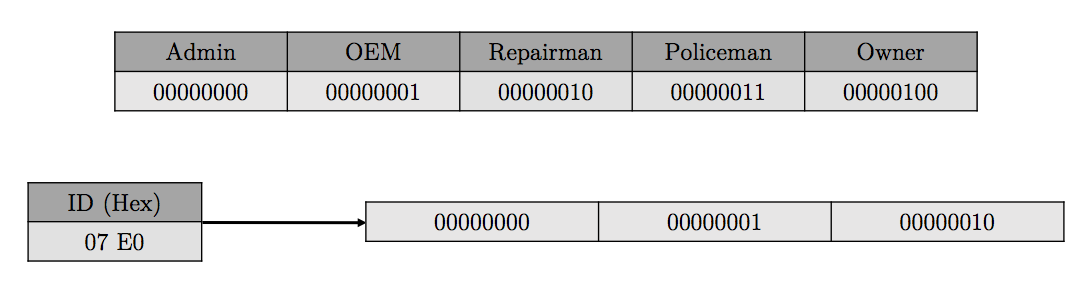
\includegraphics[width=\textwidth]{permissions.png}
	\caption{Permissions table implementation with example.}
\end{figure}